\documentclass[../../../../main.tex]{subfiles}
\begin{document}
\section*{京都大学 1978年 前期}

\subsection*{第1問}
[解] $\alpha = a+b, \beta = ab$ とする.

(与式) $\Leftrightarrow (\alpha+c) - 3\sqrt[3]{|\beta|} \cdot c^{\frac{1}{3}} - (\alpha - 2\sqrt{|\beta|}) \ge 0 \quad \cdots$ ①

この左辺を $f(c)$ とおくと $\therefore f'(c) = 1 - \sqrt[3]{|\beta|} \cdot c^{-\frac{2}{3}}$ より下表をえる

\begin{center}
\begin{tabular}{|c|c|c|c|c|}
\hline
$c$ & $0$ & $\cdots$ & $\sqrt{|\beta|}$ & $\cdots$ \\
\hline
$f'$ & & $-$ & $0$ & $+$ \\
\hline
$f$ & & $\searrow$ & & $\nearrow$ \\
\hline
\end{tabular}
\end{center}

よって,
\[ f(c) \ge f(\sqrt{|\beta|}) = \alpha + \sqrt{|\beta|} - 3\sqrt{|\beta|} - \alpha + 2\sqrt{|\beta|} = 0 \]
だから①は示された \qed


\subsection*{第2問}
[解] 点Xに対し, $\overrightarrow{OX} = \vec{x}$ とおく. $\vec{a}$ と $\vec{b}$ は一次独立.
\[ \vec{g} = \frac{1}{3}(\vec{a} + \vec{b}) \]
\[ \vec{p} = h\vec{a} \]
\[ \vec{q} = k\vec{b} \]
従って, 直線PQ上の点Xは, $t \in \mathbb{R}$ として
\[ \vec{x} = t h\vec{a} + (1-t) k\vec{b} \]
とおける. これがGを通るので,
\[ th = (1-t)k = \frac{1}{3} \]
をみたす $t \in \mathbb{R}$ が存在するから, ($h, k \neq 0$ が必要で)
\[ \frac{1}{h} + \frac{1}{k} = 3 \quad \cdots (i) \]
さらに, $T = hkS \cdots$ ① である. $\alpha = h+k$ とおく. (i)をみたす
$(h, k) (0 < h, k \le 1)$ は右図太線部.
従って, (i)から $hk = \frac{1}{3}(h+k) = \frac{1}{3}\alpha$ に注意して, 図でこれらが交点を持つ条件から
\[ \frac{1}{3}\left(\frac{2}{3} + \frac{2}{3}\right) \le \frac{1}{3}\alpha \le \frac{1}{3}\left(1 + \frac{1}{2}\right) \]
\[ \frac{4}{9} \le \frac{1}{3}\alpha \le \frac{1}{2} \]
①に代入して
\[ \frac{4}{9}S \le T \le \frac{1}{2}S \quad \text{\qed} \]

\begin{center}
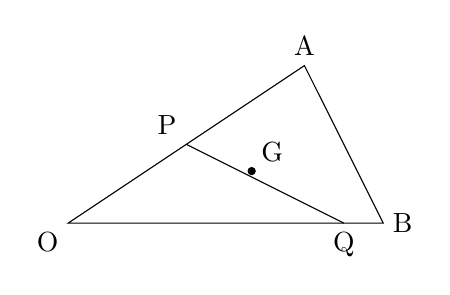
\begin{tikzpicture}
\draw (0,0) node[below left]{O} -- (3,2) node[above]{A} -- (4,0) node[right]{B} -- cycle;
\draw (1.5,1) node[above left]{P};
\draw (3.5,0) node[below]{Q};
\draw (1.5,1) -- (3.5,0);
\node at (2.33,0.66) [above right] {G};
\fill (2.33,0.66) circle (1.5pt);
\end{tikzpicture}
\end{center}

\begin{center}
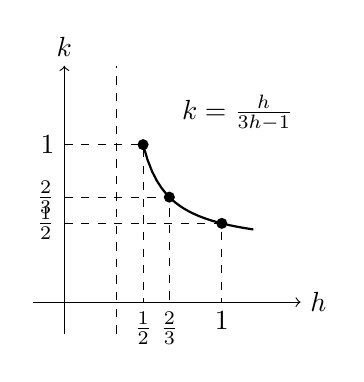
\begin{tikzpicture}[scale=2]
\draw[->] (-0.2,0) -- (1.5,0) node[right]{$h$};
\draw[->] (0,-0.2) -- (0,1.5) node[above]{$k$};
\draw[dashed] (1/3,-0.2) -- (1/3,1.5);
\draw[domain=0.5:1.2, thick] plot (\x, {\x/(3*\x-1)});
\draw[dashed] (0,1/2) node[left]{$\frac{1}{2}$} -- (1,1/2) -- (1,0) node[below]{$1$};
\draw[dashed] (0,1) node[left]{$1$} -- (1/2,1) -- (1/2,0) node[below]{$\frac{1}{2}$};
\draw[dashed] (0,2/3) node[left]{$\frac{2}{3}$} -- (2/3,2/3) -- (2/3,0) node[below]{$\frac{2}{3}$};
\fill (1,1/2) circle (1pt);
\fill (1/2,1) circle (1pt);
\fill (2/3,2/3) circle (1pt);
\node at (1.1, 1.2) {$k = \frac{h}{3h-1}$};
\end{tikzpicture}
\end{center}

\subsection*{第3問}
[解] (1) $P(t, 4-t^2)$ とおく. ($-4 \le t \le 1$)
$\triangle PAB = \frac{1}{2} \overline{AB} \cdot (P \text{と} AB \text{のキョリ})$
だから, $P$ と $AB$ のキョリ $l$ が最大の時, $\triangle PAB$ の面積も最大.
\[ l = \frac{|3t - (4-t^2)|}{\sqrt{9+1}} = \frac{|t^2 + 3t - 4|}{\sqrt{10}} = \frac{\sqrt{10}}{10} \left| \left(t+\frac{3}{2}\right)^2 - \frac{25}{4} \right| \]
より, $\max l = \frac{\sqrt{10}}{10} \cdot \frac{25}{4}$ ($t = -\frac{3}{2}$ の時) だから
もとめる $P(p, q)$ は $P\left(-\frac{3}{2}, \frac{7}{4}\right)$ \qed

(2) 題意の直線は $y = 3x + \alpha$ とおける ($\alpha \in \mathbb{R}$). これと放物線の交点の $x$ 座標は
\[ x^2 + 3x + \alpha - 4 = 0 \]
の2解であり, $x = \frac{1}{2}\left(-3 \pm \sqrt{25 - 4\alpha}\right)$ だから, $CD$ の中点 $M$ の
$x$ 座標は $x = -\frac{3}{2}$ となる. したがって(1)から, 線分 $CD$ は $x = p$ で
2等分される. \qed

(3) 右図のように面積をおく ($S = S_1 + S_2$)
\[ S = \int_{-4}^{1} (4 - x^2 - 3x) dx = \frac{1}{6} 5^3 \]
\[ S_1 = \int_{-4}^{-\frac{3}{2}} (4 - x^2 - 3x) dx = -\frac{1}{3}\left(\frac{5}{2}\right)^3 + \frac{5}{2}\left(\frac{5}{2}\right)^2 = \frac{1}{12} 5^3 \]
よって $S_1 = S_2$ となるから示された \qed

\begin{center}
\begin{tikzpicture}
\draw[->] (-5,0) -- (2,0) node[right]{$x$};
\draw[->] (0,-3) -- (0,5) node[above]{$y$};
\draw[domain=-4.5:1.5, thick] plot (\x, {4-\x*\x}) node[right]{$y=4-x^2$};
\draw[domain=-1.5:1.5, thick] plot (\x, {3*\x}) node[right]{$y=3x$};
\end{tikzpicture}
\end{center}

\subsection*{第4問}
（白紙）

\subsection*{第5問}
[解] (1) 条件は $\alpha, \beta, \gamma \in \mathbb{Z} (\alpha \le \beta \le \gamma)$ として
$f(x) = (x-\alpha)(x-\beta)(x-\gamma)$ とおけること.
$\begin{cases}
m = -(\alpha + \beta + \gamma) \\
n = \beta\gamma + \gamma\alpha + \alpha\beta \\
2 = -\alpha\beta\gamma
\end{cases}$
より, $(\alpha, \beta, \gamma) = (-2, -1, -1), (-2, 1, 1), (-1, 1, 2)$ で
あるから各々代入して
$(m, n) = (4, 5), (0, -3), (2, -1)$ \qed

(2) $k \in \mathbb{Z}$ を解に持つ時
$k(k^2 + mk + n) = -2$
$k, k^2 + mk + n \in \mathbb{Z}$ から
$(k, k^2 + mk + n) = (-2, 1), (2, -1), (1, -2), (-1, 2)$
である.
①の時 $k = -2, 3 - 2m + n = 0$
②の時 $k = 2, 5 + 2m + n = 0$
③の時 $k = 1, 3 + m + n = 0$
④の時 $k = -1, -1 - m + n = 0$
逆にこの時 $k$ がみたされて, 十分である. \qed

(3) (2)から条件は
$n = 2m - 3, n = -2m - 5, n = -m - 3, n = m + 1$
$|m|, |n| \le 5$
だから図示して下図

\begin{center}
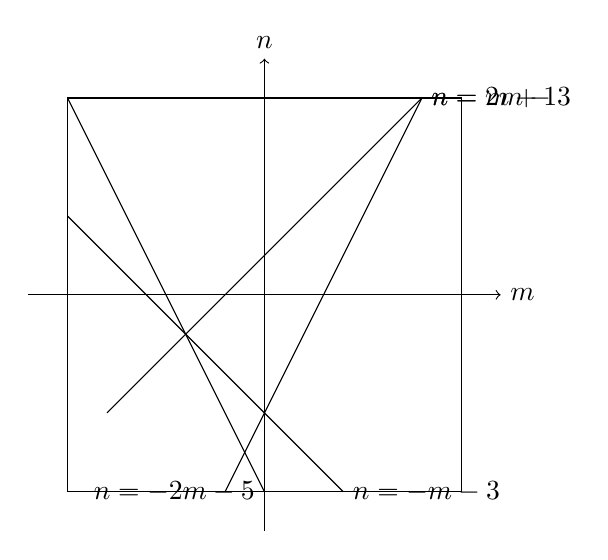
\begin{tikzpicture}[scale=0.5]
\draw[->] (-6,0) -- (6,0) node[right]{$m$};
\draw[->] (0,-6) -- (0,6) node[above]{$n$};
\draw (-5,-5) rectangle (5,5);
\draw[domain=-1:4] plot (\x, {2*\x - 3}) node[right]{$n=2m-3$};
\draw[domain=-5:0] plot (\x, {-2*\x - 5}) node[left]{$n=-2m-5$};
\draw[domain=-5:2] plot (\x, {-\x - 3}) node[right]{$n=-m-3$};
\draw[domain=-4:4] plot (\x, {\x + 1}) node[right]{$n=m+1$};
\end{tikzpicture}
\end{center}

よって $(m, n)$ の組数は
$10 + 8 + 6 + 6 - 4 = 26$ コ

\subsection*{第6問}
[解] (i) $\cos(m+n)x = \cos mx \cos nx - \sin mx \sin nx$ (複合同順) の辺々引いて,
$\frac{1}{2} \{ \cos(m-n)x - \cos(m+n)x \} = \sin mx \sin nx$ \qed
したがって,
\[ I_{m,n} = \frac{1}{2} \int_{-\pi}^{\pi} \{ \cos(m-n)x - \cos(m+n)x \} dx \]
\[ = \begin{cases} 0 & (m \neq n) \\ \pi & (m = n) \end{cases} \quad \text{\qed} \]

(ii) 被積分関数を $g_k(x)$ とおく.
\[ g_k(x) = \sin^2 kx - 2(a \sin mx + b \sin nx) \sin kx + (a \sin mx + b \sin nx)^2 \]
\[ = \sin^2 kx + a^2 \sin^2 mx + b^2 \sin^2 nx + 2ab \sin mx \sin nx - 2(a \sin mx + b \sin nx) \sin kx \]
から, (i) より
\[ f(0) = \pi(a^2+b^2) + 2ab I_{m,n} \]
\[ f(k) = \pi(a^2+b^2+1) + 2ab I_{m,n} - 2a I_{m,k} - 2b I_{n,k} \quad (k \ge 1) \]
$5 C_0 = 5 C_5 = 1, 5 C_1 = 5 C_4 = 5, 5 C_2 = 5 C_3 = 10$ だから,
\[ E = \left(\frac{1}{2}\right)^5 \left[ \pi(32a^2 + 32b^2 + 31) + 64ab I_{m,n} - 2a \sum_{k=0}^{5} {}_5C_k I_{m,k} - 2b \sum_{k=0}^{5} {}_5C_k I_{n,k} \right] \]
ここで, $m, n \in \mathbb{N}$ 及び $0 \le k \le 5$ から,
$\sum_{k=0}^{5} {}_5C_k I_{m,k} = \begin{cases} {}_5C_m \cdot \pi & (1 \le m \le 5 \text{ の時}) \\ 0 & (6 \le m \text{ の時}) \end{cases}$
である. 又, $m$ の部を $A$ とおく.

$1^\circ \ m=n \text{ の時}$
$I_{m,n} = \pi$ だから,
$E = \frac{1}{32} [ 32(a+b)^2 + 31 ] \pi \quad (6 \le m)$
$E = \frac{1}{32} [ 32(a+b)^2 - 2(a+b) {}_5C_m + 31 ] \pi \quad (1 \le m \le 5)$
である. $6 \le m$ の時, $a+b=0$ で $\min E = \frac{31}{32}\pi$ をとる.
$1 \le m \le 5$ の時, $a+b = \frac{{}_5C_m}{32}$ で $\min E = \frac{\pi}{32} \left( 31 - \frac{({}_5C_m)^2}{32} \right)$ をとる. ③から
$m=2$ 又は $3$ の時, $\min E$ は最小値 $\frac{223}{256}\pi$ をとる.

$2^\circ \ m \neq n$
$I_{m,n} = 0$ から $A = \pi [32(a^2+b^2)+31]$ である. 対称性から $m < n$ として良い.
$2^5 \cdot E$ の値は以下のようになる.

\begin{center}
\begin{tabular}{|c|c|c|}
\hline
$n \backslash m$ & $1 \le m \le 5$ & $6 \le m$ \\
\hline
$1 \le n \le 5$ & $A - 2\pi(a \cdot {}_5C_m + b \cdot {}_5C_n)$ (⑦) & \\
\hline
$6 \le n$ & $A - 2\pi \cdot a \cdot {}_5C_m$ (ウ) & $A$ (エ) \\
\hline
\end{tabular}
\end{center}

まず, ⑦の時. $a, b \le 0$ ならば $E$ は $a, b$ の単調減少関数だから ($\because {}_5C_k > 0$)
$a=b=0$ で $\min E = \frac{31}{32}\pi$ をとる. $a, b > 0$ の時, $m < n$ だから $(m,n) = (2,3)$ で
$2^5 \frac{1}{\pi} E = 32(a^2+b^2) + 31 - 20(a+b)$
$= 32\left(a - \frac{5}{16}\right)^2 + 32\left(b - \frac{5}{16}\right)^2 + 31 - \frac{25}{4}$
$\ge \frac{99}{4}$ （等号成立は $a=b=\frac{5}{16}$）
から, $a=b=\frac{5}{16}$ で $\min E = \frac{99}{128}\pi$ をとる.

次に(ウ)の時, $a \le 0$ ならば同様に $\min E = \frac{31}{32}\pi$. $a > 0$ の時, $m=2, 3$ で,
$2^5 \frac{1}{\pi} E = 32(a^2+b^2) + 31 - 20a$
$\ge 31 - \frac{25}{8} = \frac{223}{8}$ （等号成立は $a=\frac{5}{16}, b=0$）

(エ)の時は $a=b=0$ で $\min E = \frac{31}{32}\pi$ である.

以上から, $2^\circ$ の⑦の時, 且つ $m \neq n$ で, 対称性から
$(m,n,a,b) = \left(3, 2, \frac{5}{16}, \frac{5}{16}\right), \left(2, 3, \frac{5}{16}, \frac{5}{16}\right)$ \qed

\end{document}
